\section{Численный эксперимент}

Численный эксперимент проводился с помощью программного пакета Lumerical FDTD Solutions. При этом исследовался спектр пропускания пар наностержней в виде прямоугольных параллелепипедов. Ширина и высота наностержней оставались фиксированными во всех численных расчетах и равнялись 50 нм и 30 нм, соответственно. Вид исследуемой структуры и основные элементы для проведения численного расчета показаны на рис.~\ref{img:lumerical}. 
\begin{figure}
\center{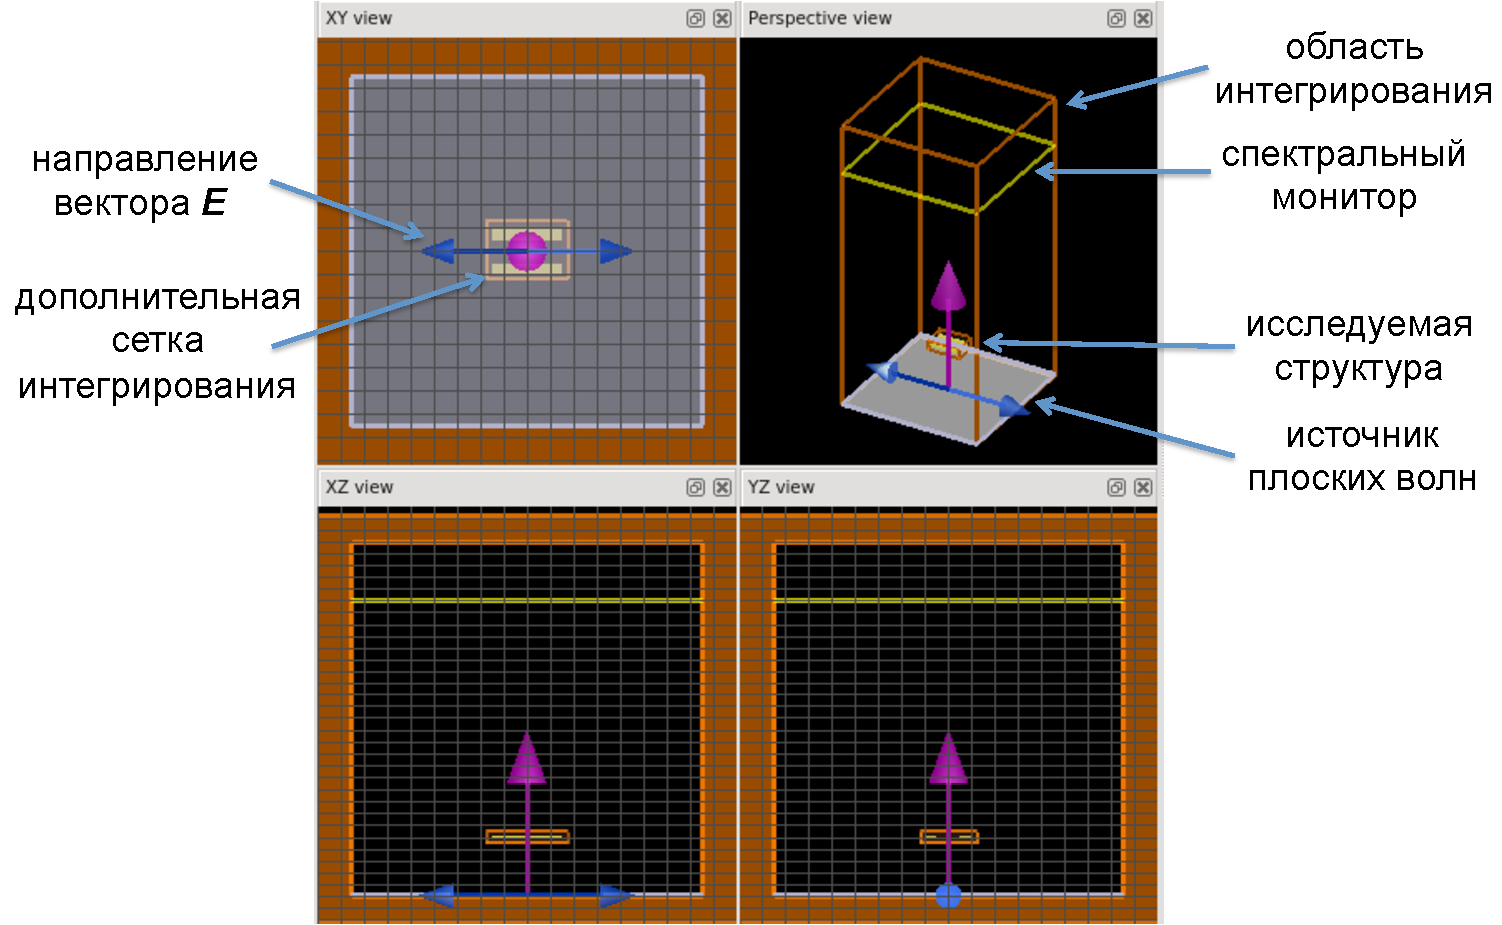
\includegraphics[width=12cm]{img/FDTD/lumerical.pdf}}
\caption{Вид исследуемой структуры и основные элементы для проведения численного расчета в программе Lumerical FDTD Solutions.}
\label{img:lumerical}
\end{figure}

Область интегрирования составляла 1.5 * 1.5 * 3 мкм$ ^3 $. Во всех пограничных плоскостях были выбраны граничные условия PML. Расчет спектра производился на расстоянии 1.5 мкм от образца для того, чтобы избежать детектирования ближнего поля. Минимальное количество узлов сетки было 22 на длину волны, которое было определено проверкой на сходимость; в дополнительной сетке расстояние между узлами сетки составляло 5 нм для улучшения точности вычислений. На образец падал фемтосекундный импульс с поляризацией, параллельной наностержням. Далее, с помощью преобразования Фурье рассчитывался спектр пропускания для различных длин волн падающего электромагнитного излучения. Характерный спектр пропускания показан на рис.~\ref{img:spectraFDTDa500d100}. Наблюдаются два резонанса: более глубокий при длине волны $ \approx 1600 $ нм  -- резонанс первого порядка, и при длине волны $ \approx 680 $ нм -- резонанс второго порядка.
\begin{figure}
\center{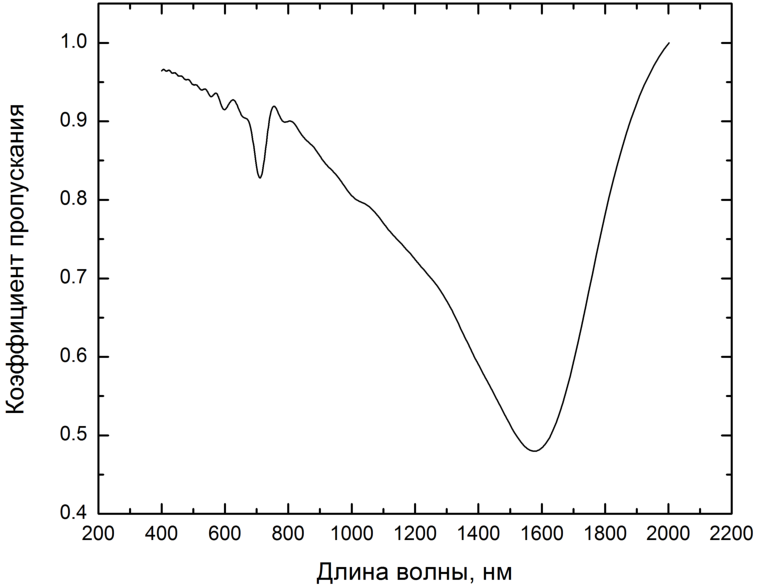
\includegraphics[width=12cm]{img/FDTD/spectra_a500d100.pdf}}
\caption{Спектр пропускания димера наностержней длиной 500 нм и расстоянием 100 нм между наностержнями, рассчитанный с помощью программного пакета Lumerical FDTD.}
\label{img:spectraFDTDa500d100}
\end{figure}

Локальное распределение плотности мощности электромагнитного поля для данных параметров пар наностержней представлено на рис.~\ref{img:locala500d100FDTD}. При этом рассчитывалось значение квадрата модуля вектора электрической напряженности $ \lvert E \rvert ^2 $ на расстоянии 20~нм от наностержней вдоль оси $ Oz $ на резонансных длинах волн. Видно, что при падении света с длиной волны 1600 нм (рис.~\ref{img:locala500d100FDTD}б) в наностержне возникает две пучности плотности мощности электромагнитного поля, а при падении света c длиной волны 680 нм (рис.~\ref{img:locala500d100FDTD}б) --- четыре пучности.

\begin{figure}
\center{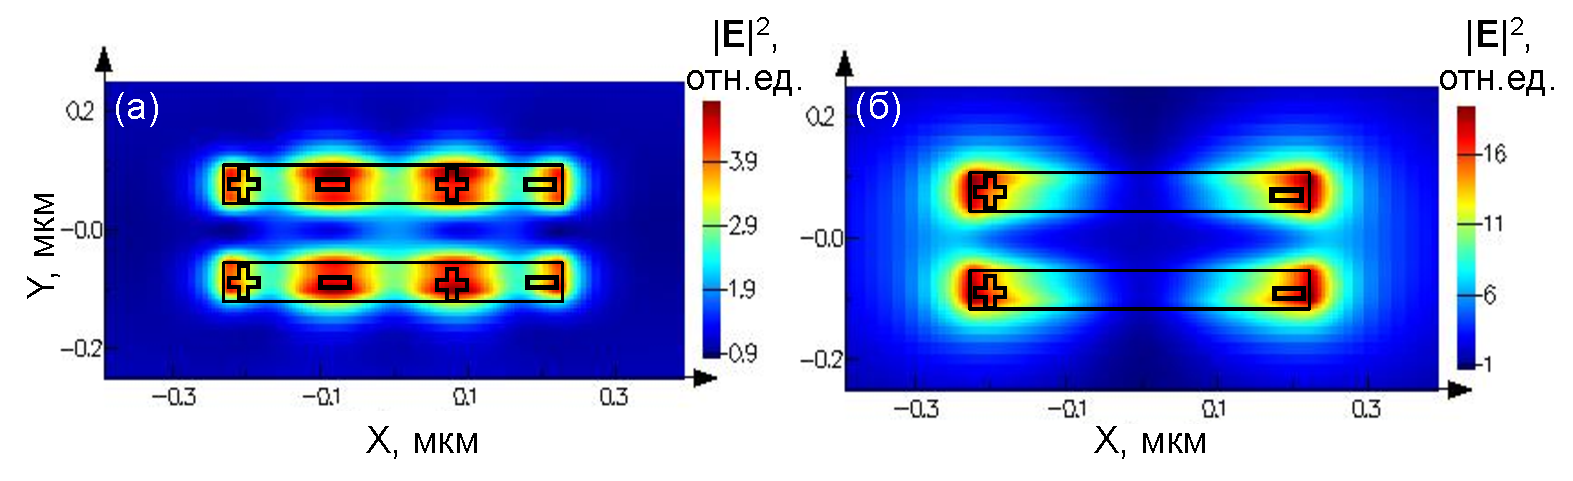
\includegraphics[width=16cm]{img/FDTD/localfield.pdf}}
\caption{Локальное распределение электромагнитного поля на расстоянии 20 нм от наностержней и мгновенное распределение зарядов при падающем электромагнитном излучении с длиной волны 680 нм (a) и 1600 нм (б).}
\label{img:locala500d100FDTD}
\end{figure}

Далее варьировалось расстояние между наностержнями фиксированной длины 500 нм от 10 нм до 650 нм с шагом 20 нм. В итоге были получены спектры пропускания для различных расстояний между наностержнями. В каждом из спектров определялись положения резонансов первого и второго порядков. Графики зависимости положения резонансов первого и второго порядков от расстояния между наностержнями представлены на рис.~\ref{img:a500PML}. На расстояниях до 150 нм график зависимости схож с графиком на рис.~\ref{img:semianalytical_dd} для случая симметричной моды. Далее начинает появляться вклад дальнепольного взаимодействия, в связи с чем кривая положения резонанса не носит монотонный характер, а появляются осцилляции. Для резонанса второго порядка кривая носит монотонный характер до $ \approx 400 $ нм, а дальше начинаются осцилляции с амплитудой $ \approx 3 $ нм. Значит, данную структуру можно использовать в качестве <<плазмонной линейки>> для резонанса первого порядка до $ \approx 150 $ нм, а для резонанса второго порядка --- до $ \approx 400 $ нм.

\begin{figure}
\center{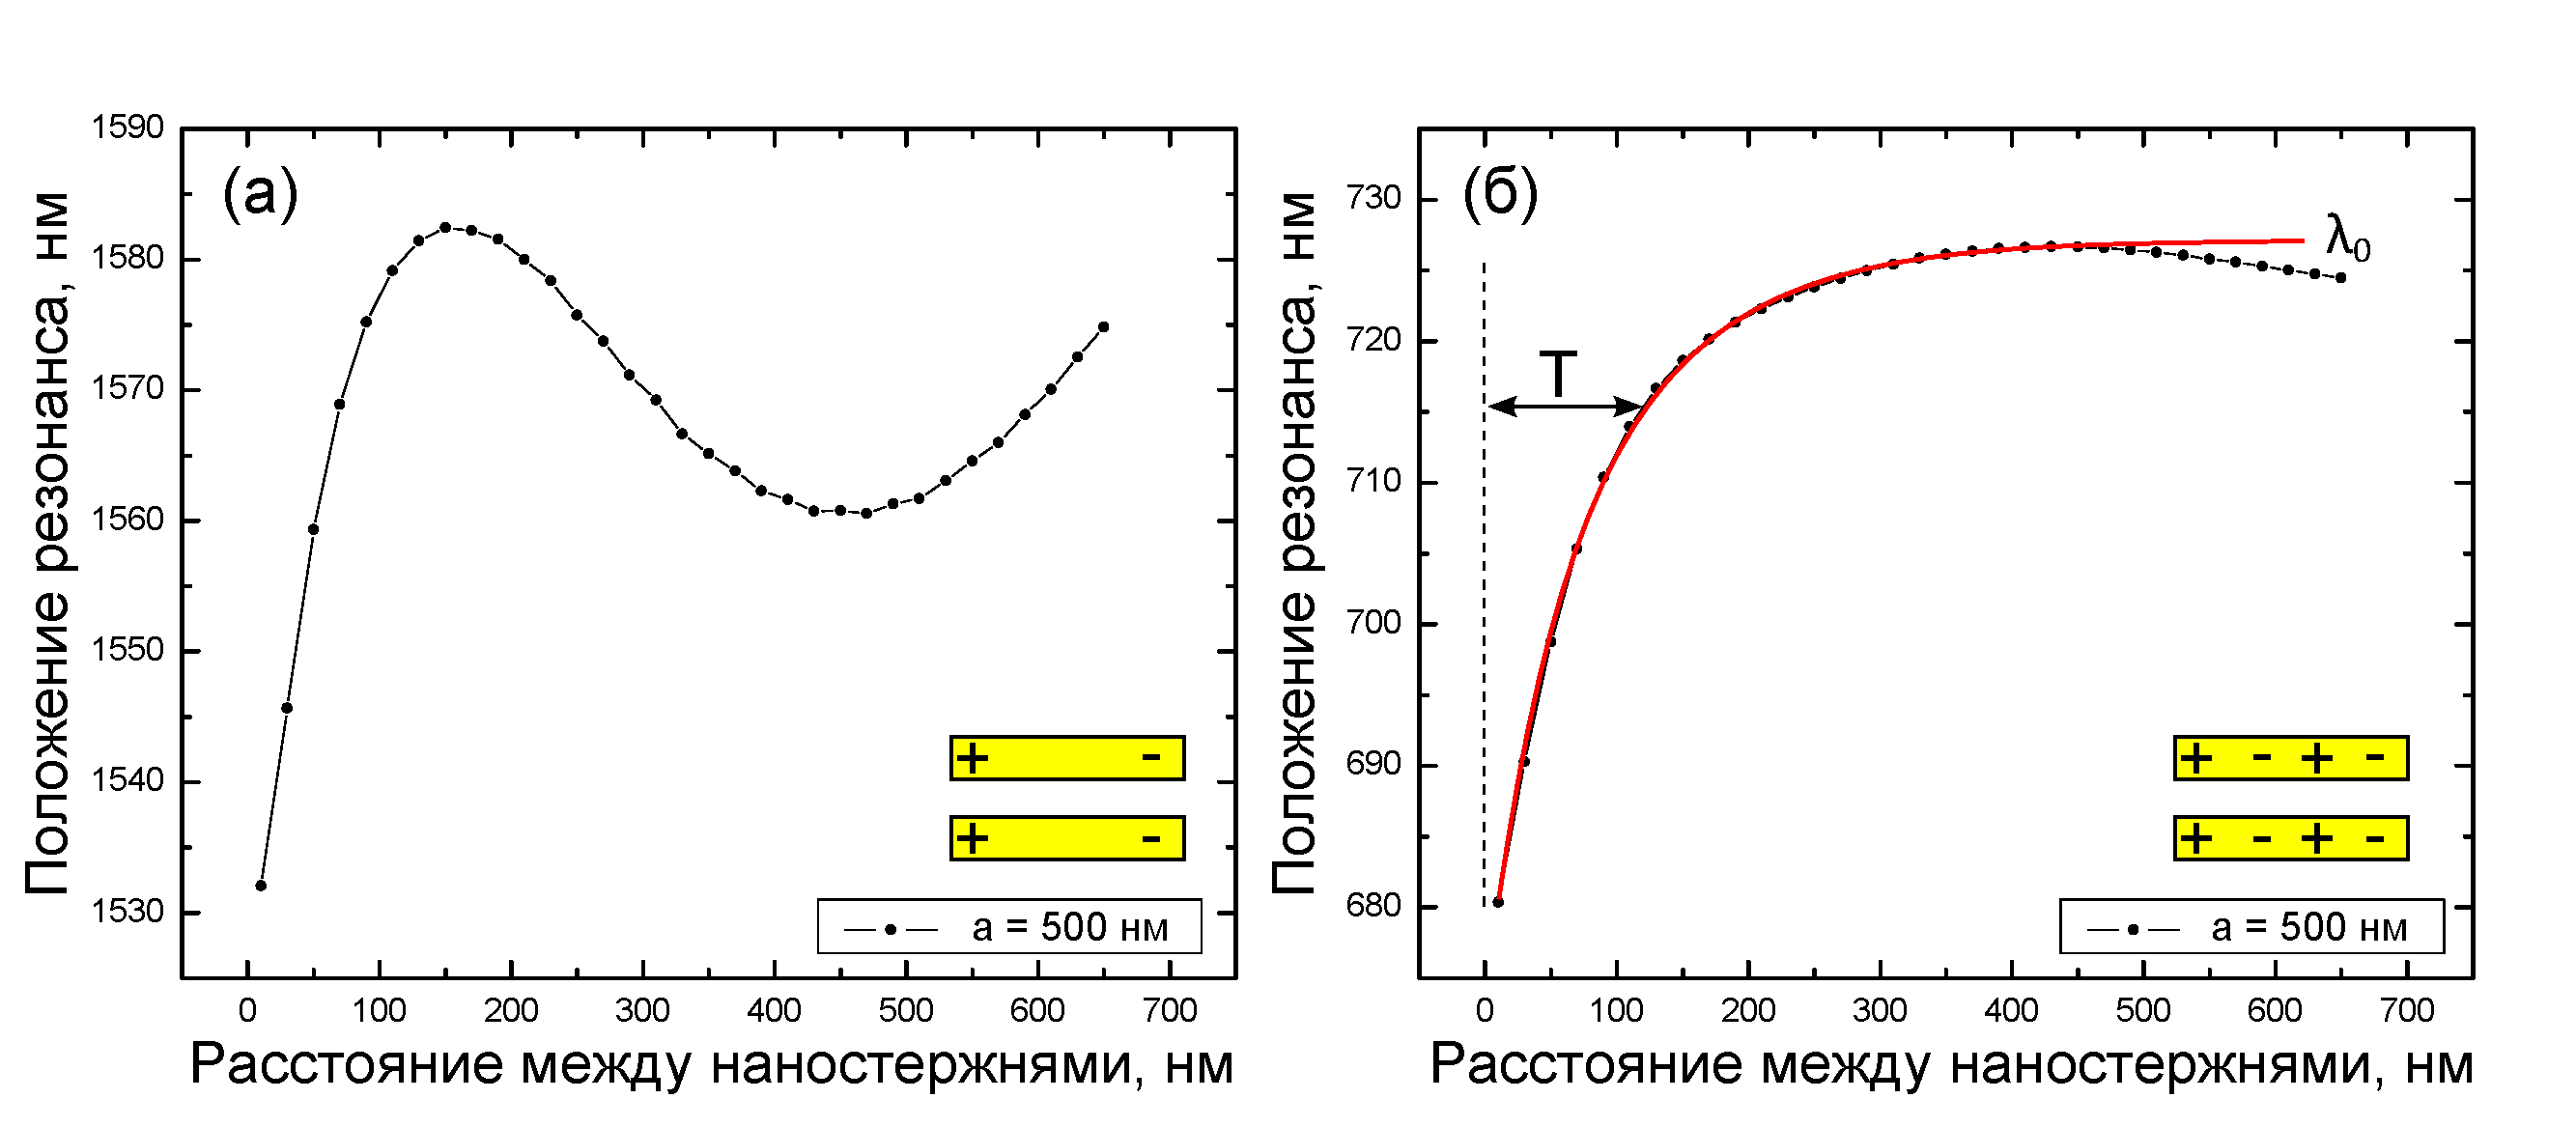
\includegraphics[width=16cm]{img/FDTD/a500PML.pdf}}
\caption{Графики зависимости положения  резонансов первого (а) и второго (б) порядков от расстояния между наностержнями длиной 500 нм. Вставки -- мгновенное распределение зарядов для резонанса первого (а) и второго (б) порядков.}
\label{img:a500PML}
\end{figure}

При уменьшении длины и фиксированном расстоянии наностержней резонансная длина волны смещалась в синюю область. На рис.~\ref{img:a300PML} показана зависимость положения резонасов от расстояния между наностержнями при их длине 300 нм. Видно, что характерные для резонансов первого и второго порядков осцилляции сохраняются, а также сохраняется значение верхней границы применимости <<плазмонной линейки>>, которая определяется равенством нуля первой производной положения резонанса от расстояния между наностержнями и составляет  $ \approx 150 \pm 10 $ нм для резонса первого порядка и $ \approx 400 \pm 30 $ нм для резонанса второго порядка.

\begin{figure}
\center{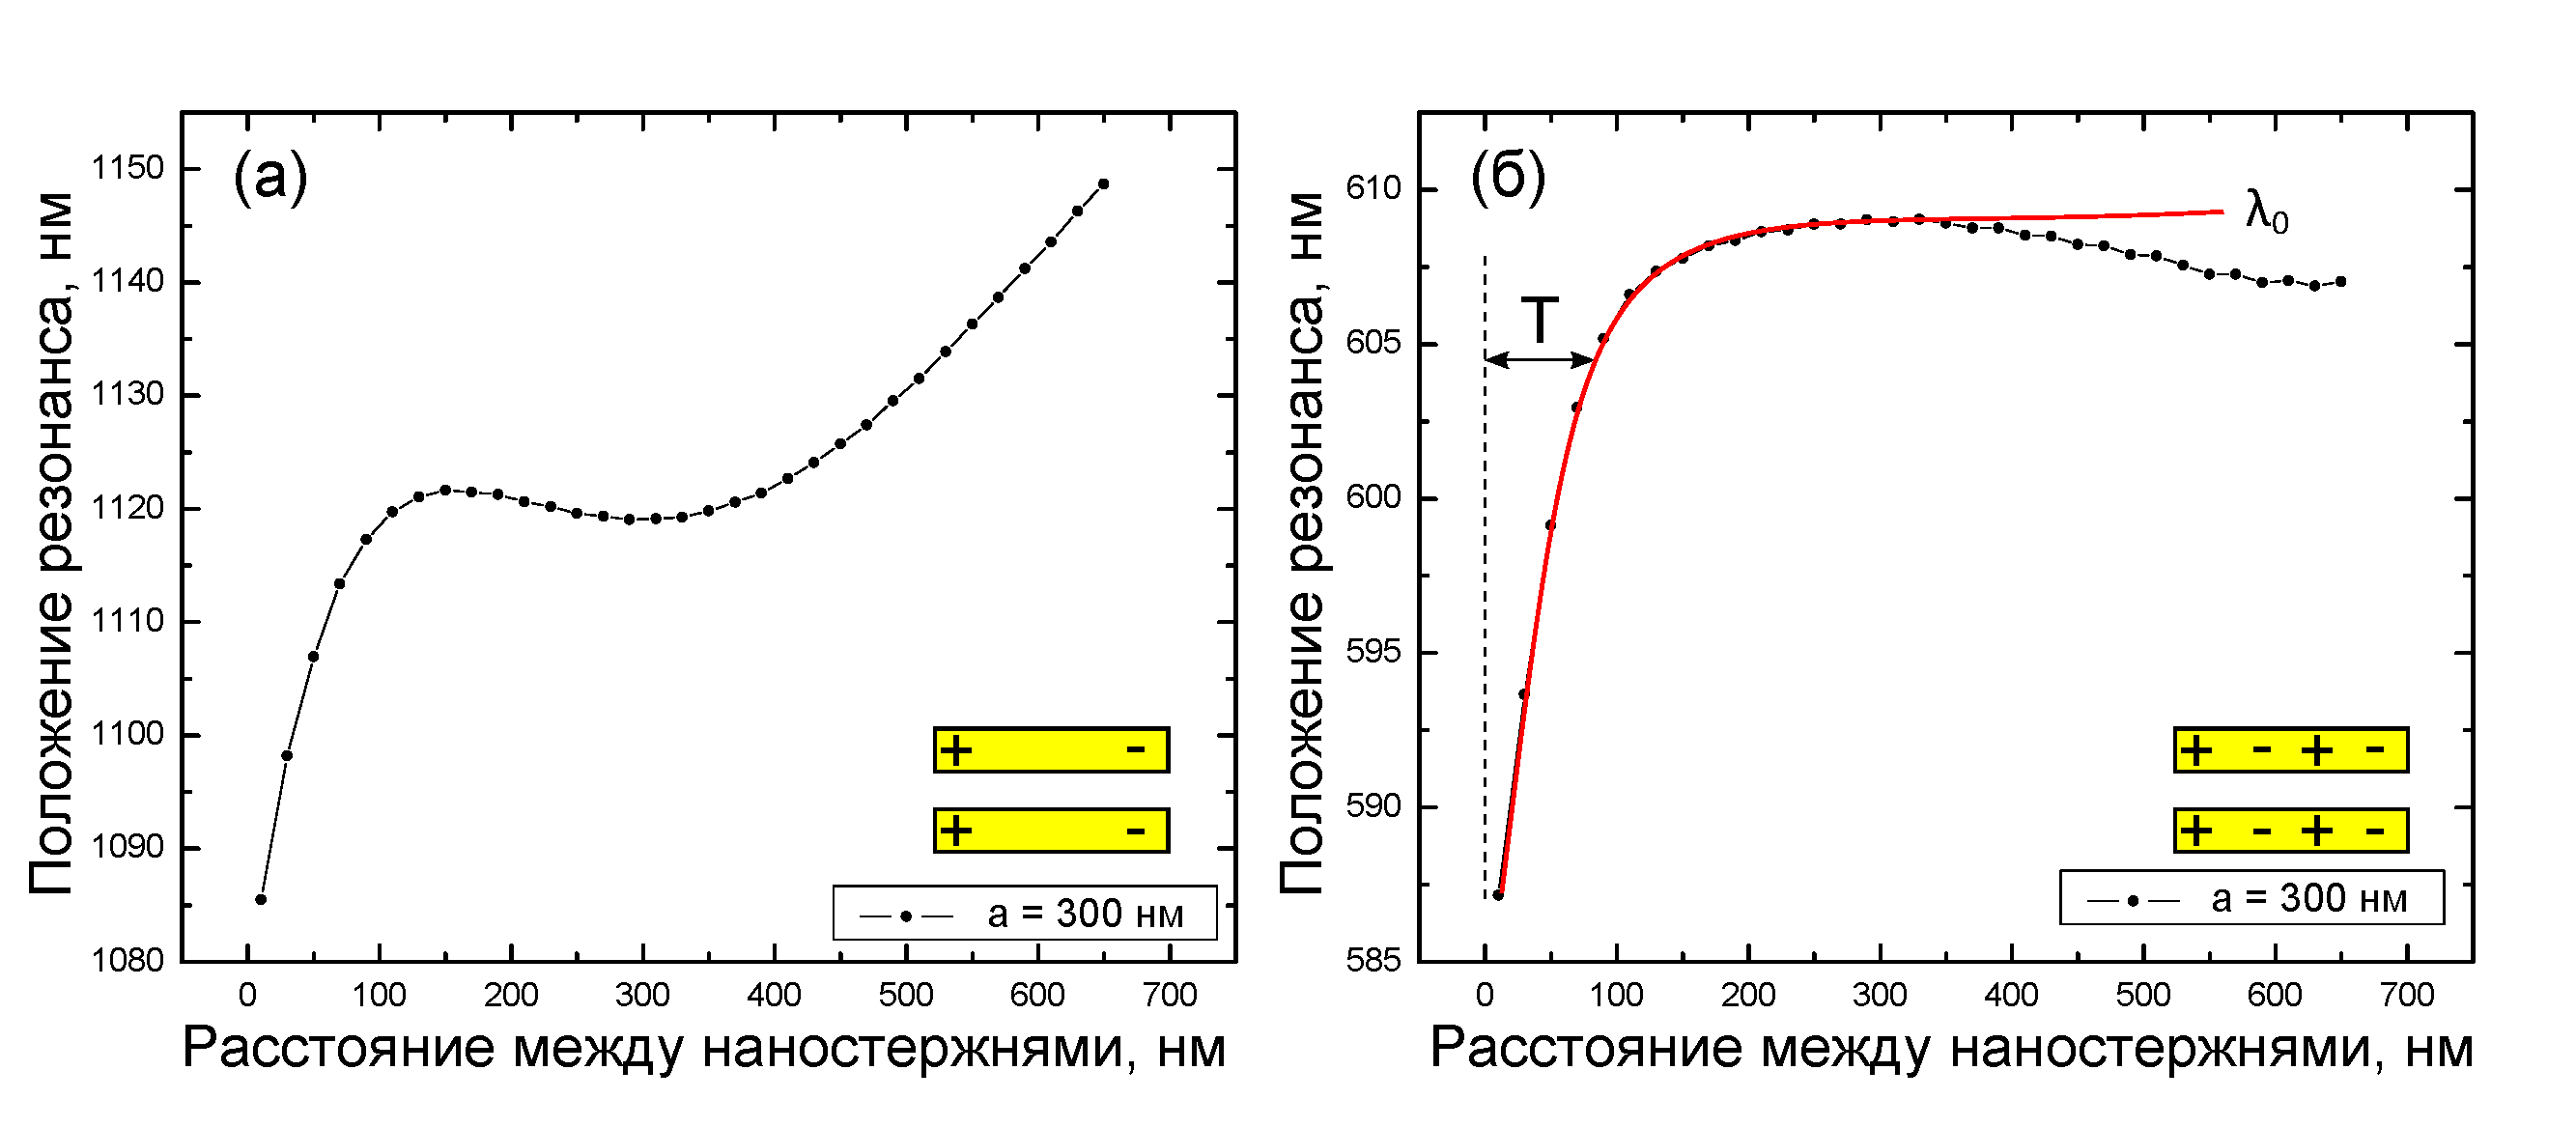
\includegraphics[width=16cm]{img/FDTD/a300PML.pdf}}
\caption{Графики зависимости положения  резонансов первого (a) и второго (б) порядков от расстояния между наностержнями длиной 300 нм. Вставки -- мгновенное распределение зарядов для резонанса первого (a) и второго (б) порядков.}
\label{img:a300PML}
\end{figure}

Далее рассчитывался спектр пропускания для пар наностержней длиной от 100 нм до 500 нм с шагом 50 нм, и для каждой фиксированной длины наностержней рассчитывалась зависимость положения резонанса первого и второго порядков от расстояния между наностержнями. При этом резонанс второго порядка становится различным при длине наностержней 250 нм и больше. Данная зависимость положения резонансов от расстояния между наностержнями аппроксимировалась экспонентой вида $ y(x) = A \exp (-x/ T ) + y_0 $ . График зависимости постоянной затухания $ T $ от длины наностержней показан на рис.~\ref{img:expdecay}а для резонанса первого порядка и на рис.~\ref{img:expdecay}б для резонанса второго порядка.

\begin{figure}
\center{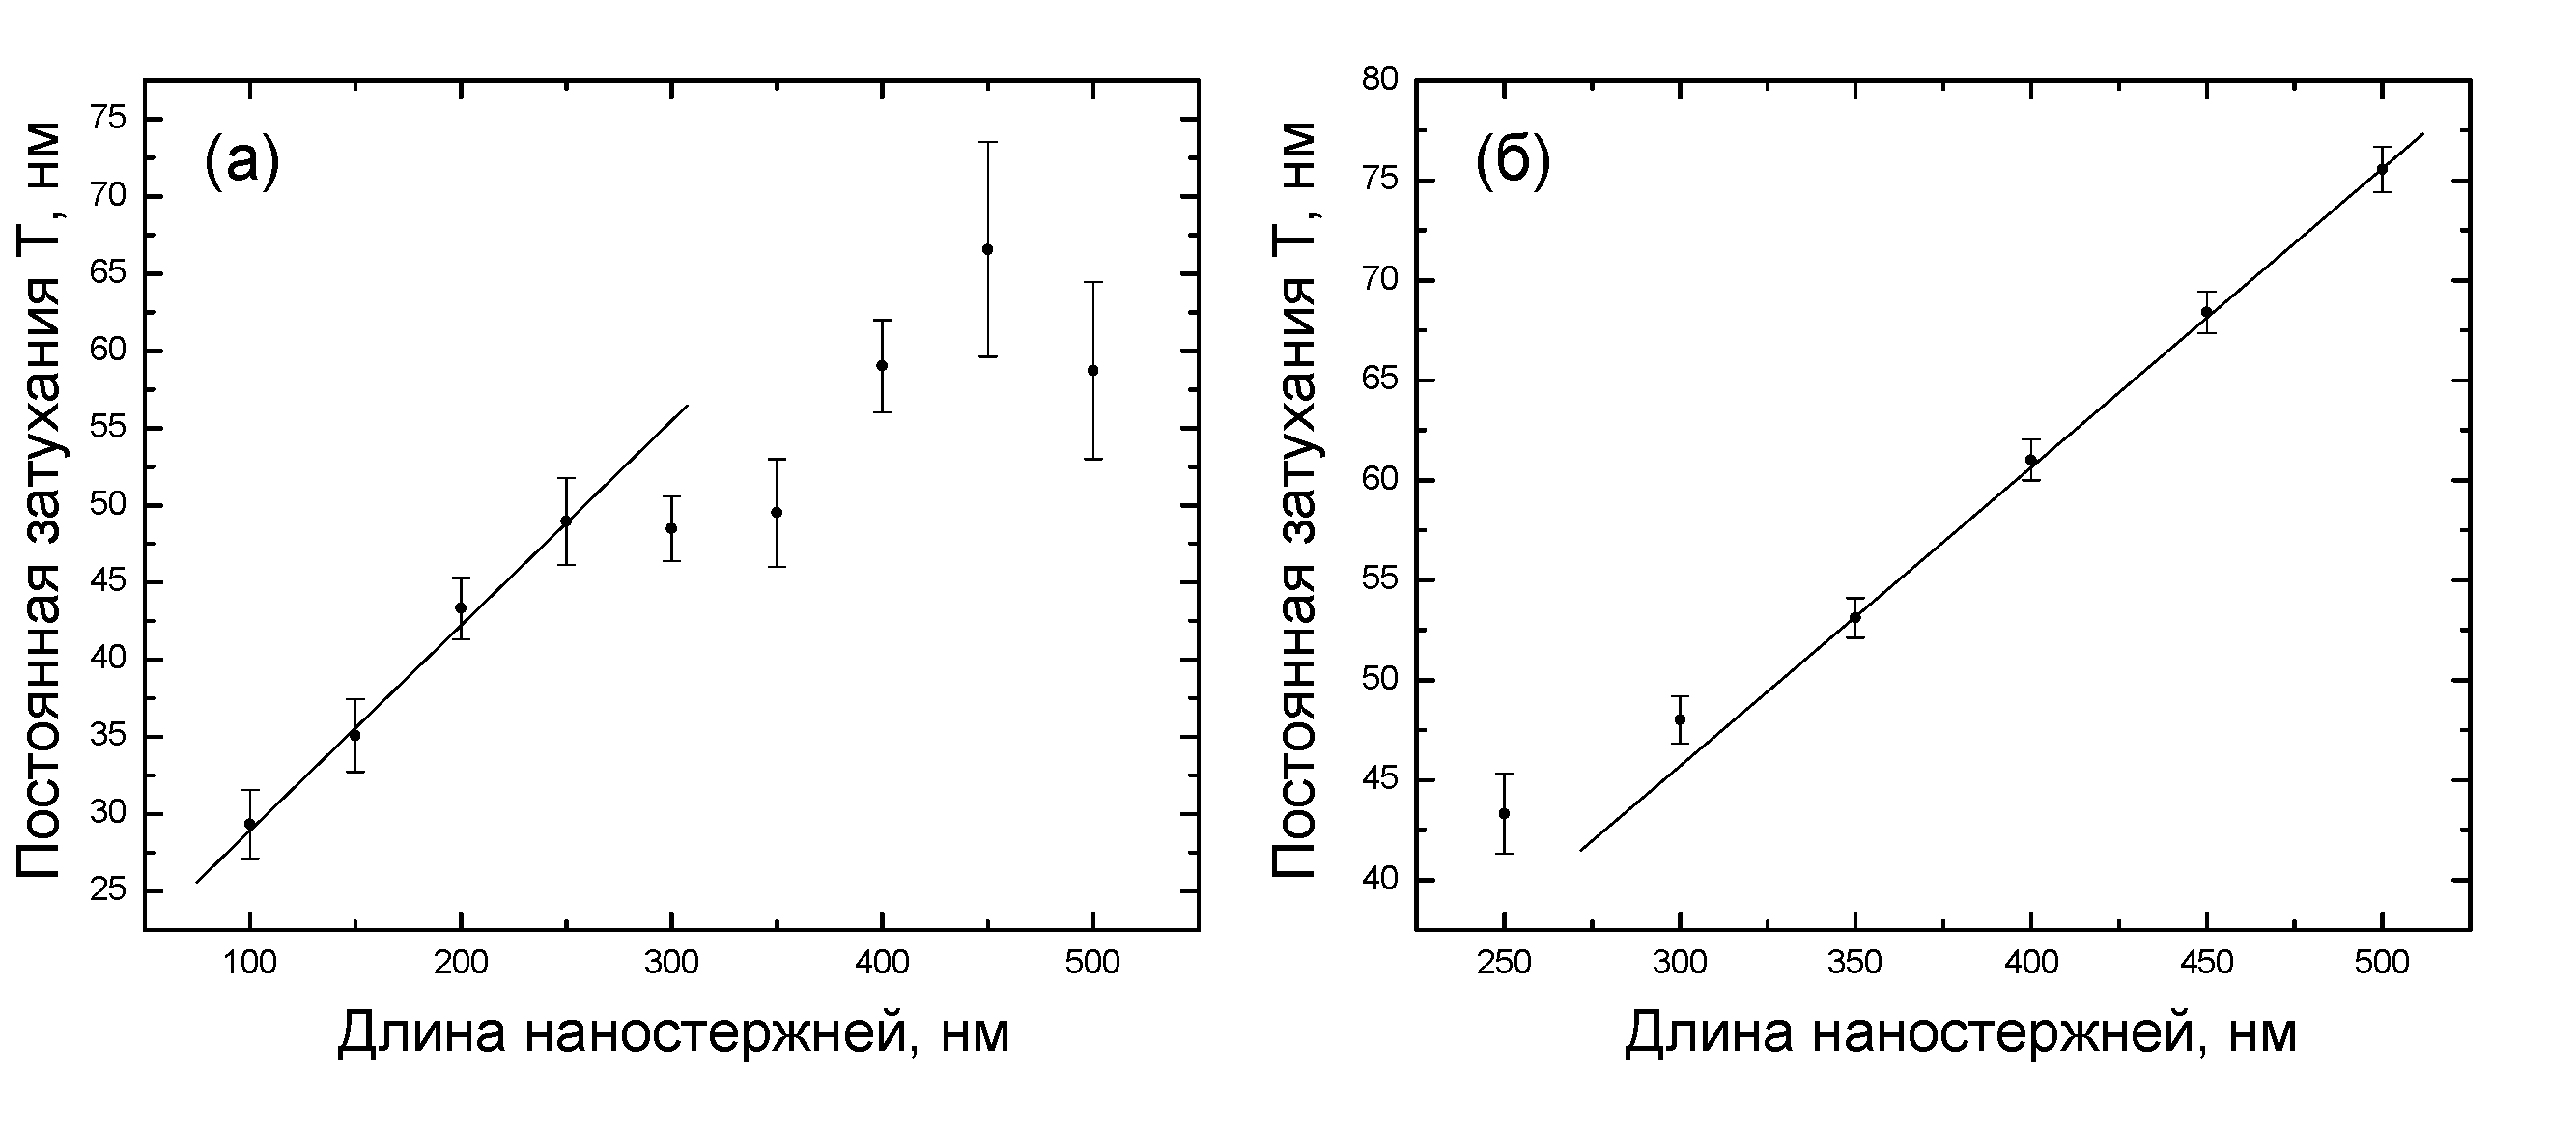
\includegraphics[width=16cm]{img/FDTD/expdecay.pdf}}
\caption{Графики зависимости значения постоянной затухания $ T $ от длины наностержней для резонанса первого порядка (а) и для резонанса второго порядка (б).}
\label{img:expdecay}
\end{figure}

Из графиков видно, что линейная зависимость сохраняется для резонансов первого порядка при длине наностержней от 100 нм до 250 нм, а для резонанса второго порядка при длине наностержней от 350 нм до 500 нм. Значит, для уравнения <<плазмонной линейки>> положение резонанса первого порядка можно использовать для длин наностержней от 100 нм до 250 нм  , а положение резонанса второго порядка --- для длин наностержней от 350 нм до 500 нм.

Пусть $ \lambda_0 $ -- резонансная длина волны, которая определяется соотношением
\begin{equation}
\dfrac{\partial \lambda}{\partial d} \Big|_{\lambda _0} = 0,
\end{equation}
где $ \lambda $ -- длина волны резонанса первого или второго порядков, $ d $ -- расстояние между наностержнями. Тогда график сдвига резонанса первого порядка $ \Delta \lambda =  \lambda - \lambda_0 $ от расстояния между наностержнями для различных длин наностержней показан на рис.~\ref{img:ruler1}а. Далее расстояние нормировалось на геометрический параметр наностержней с размерностью длины, и если расстояние нормировать на квадратный корень из площади $ S $ наностержня, то получается уравнение для <<плазмонной линейки>>:
\begin{equation}
\frac{\Delta \lambda}{\lambda_0} \approx 0.044 \exp \left( - 2.38 \frac{d}{\sqrt{S}} \right).
\label{eq:ruler1}
\end{equation}
График кривой, описывающейся уравнением (\ref{eq:ruler1}), показан на рис.~\ref{img:ruler1}б сплошной черной линией, а точками показаны положения относительного сдвига резонансов первого порядка для наностержней с длиной 100, 150, 200 и 250 нм.

\begin{figure}
\center{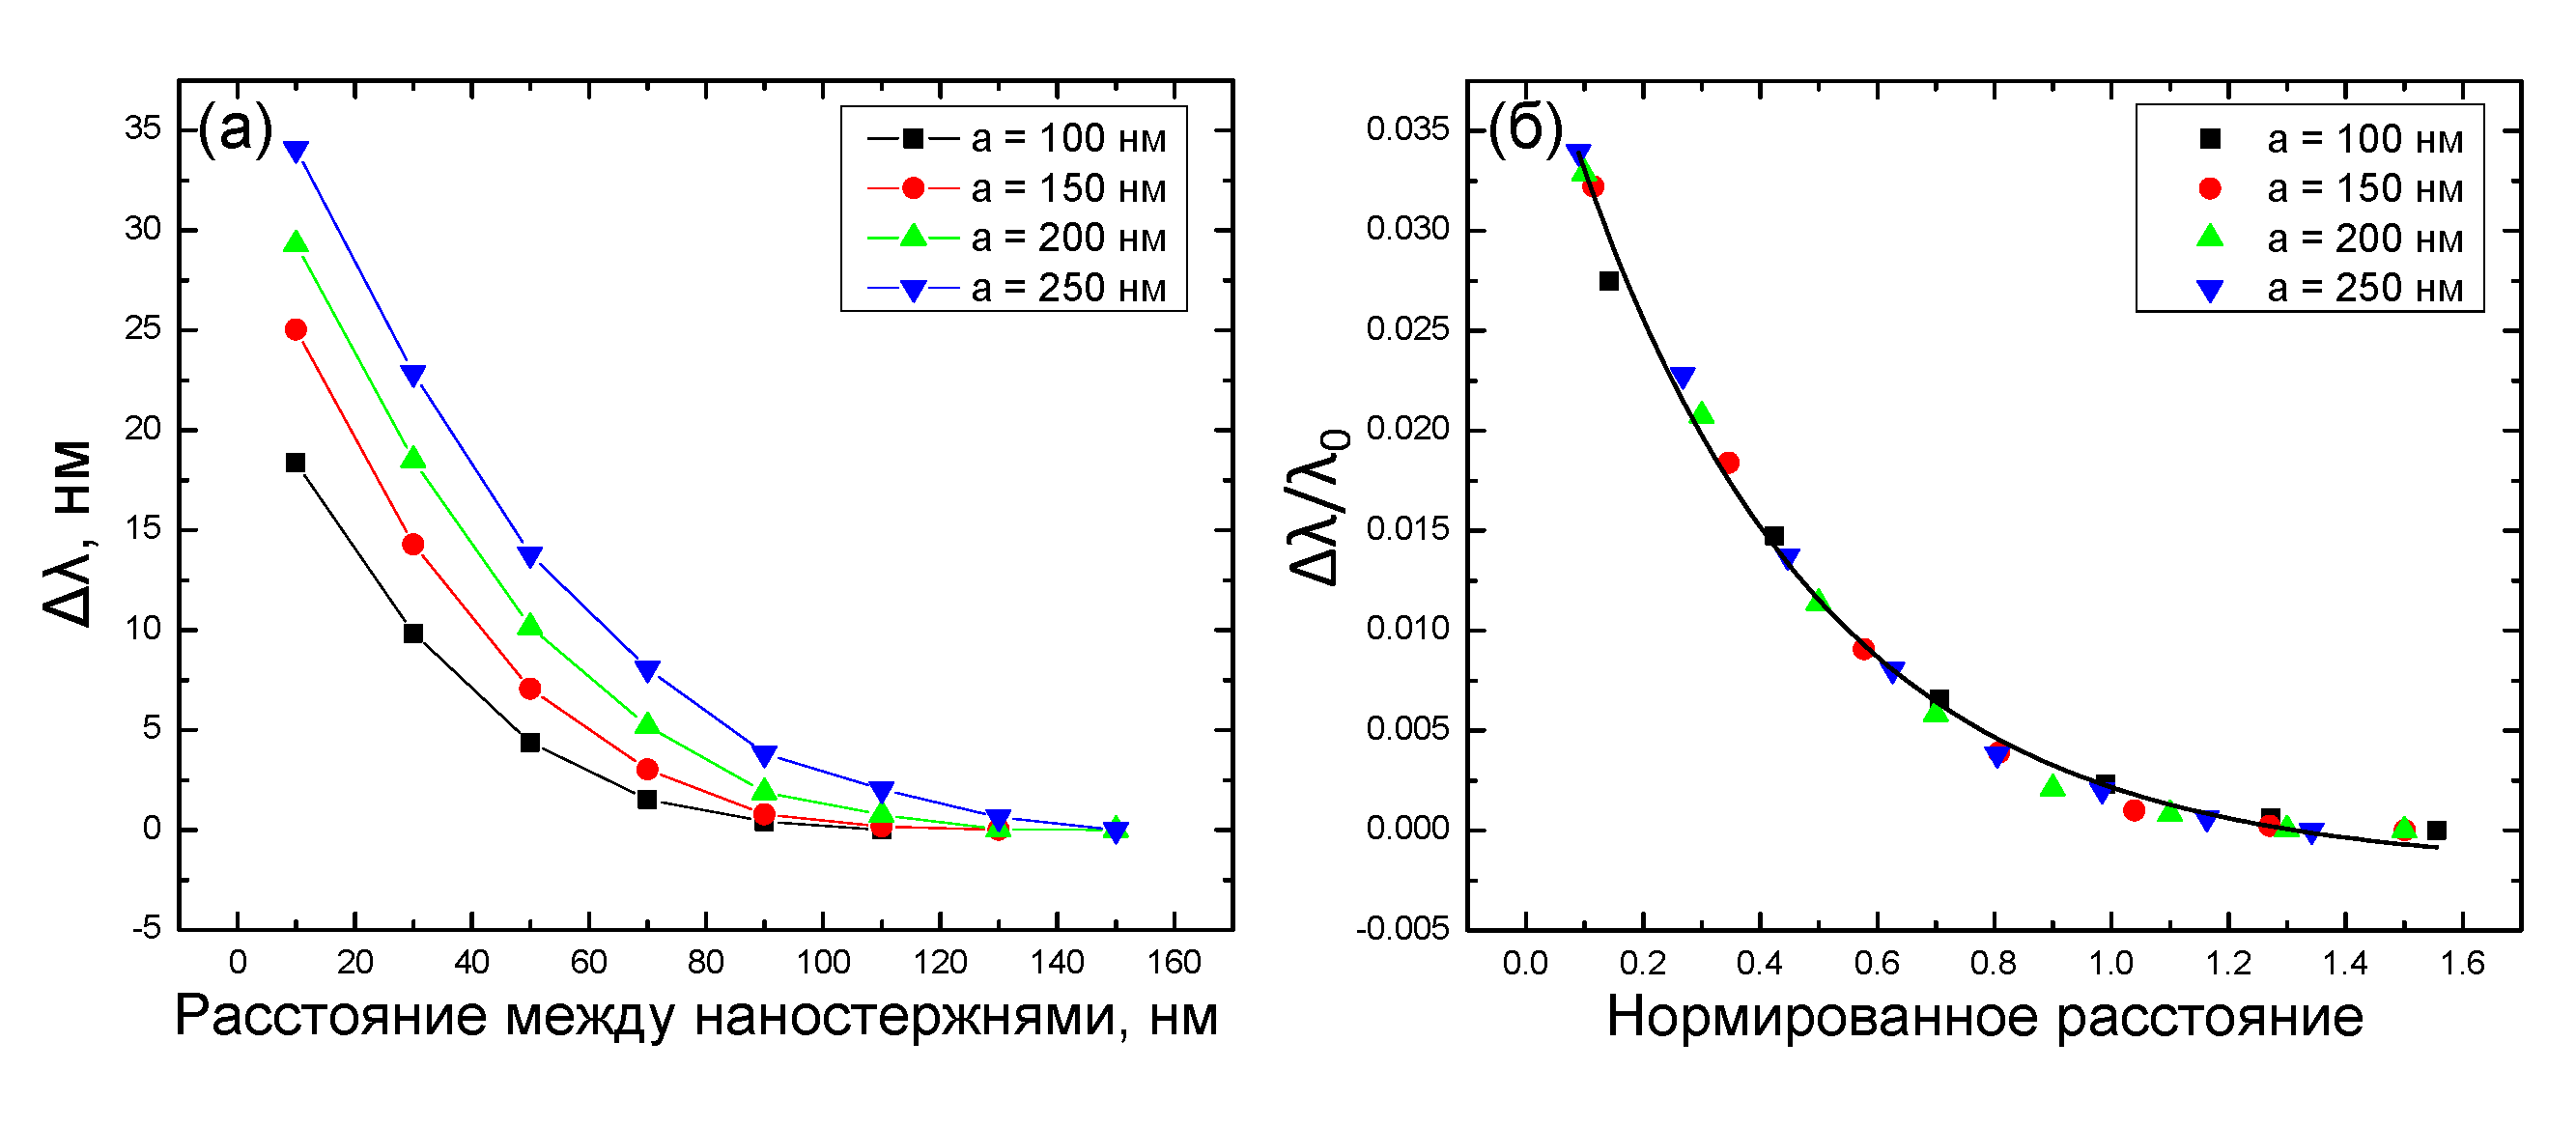
\includegraphics[width=16cm]{img/FDTD/ruler_res1.pdf}}
\caption{Графики зависимости сдвига резонанса первого порядка $ \Delta \lambda $ от расстояния между наностержнями (а) и зависимость относительного сдвига резонанса первого порядка от нормированного на квадратный корень из площади наностержня расстояния (б) при длине наностержней 100, 150, 200 и 250 нм. }
\label{img:ruler1}
\end{figure}

Для резонанса второго порядка также можно получить уравнение <<плазмонной линейки>>, если расстояние между наностержнями нормировать на длину наностержней $ a $. Тогда уравнение выглядит следующим образом:
\begin{equation}
\frac{\Delta \lambda}{\lambda_0} \approx 0.063 \exp \left( - 6.62 \frac{d}{a} \right).
\end{equation}
Графики зависимости сдвига резонанса второго порядка $ \Delta \lambda $ от расстояния между наностержнями и зависимость относительного сдвига резонанса второго порядка от нормированного расстояния при длине наностержней 350, 400, 450 и 500 нм показаны на рис.~\ref{img:ruler2}.

\begin{figure}
\center{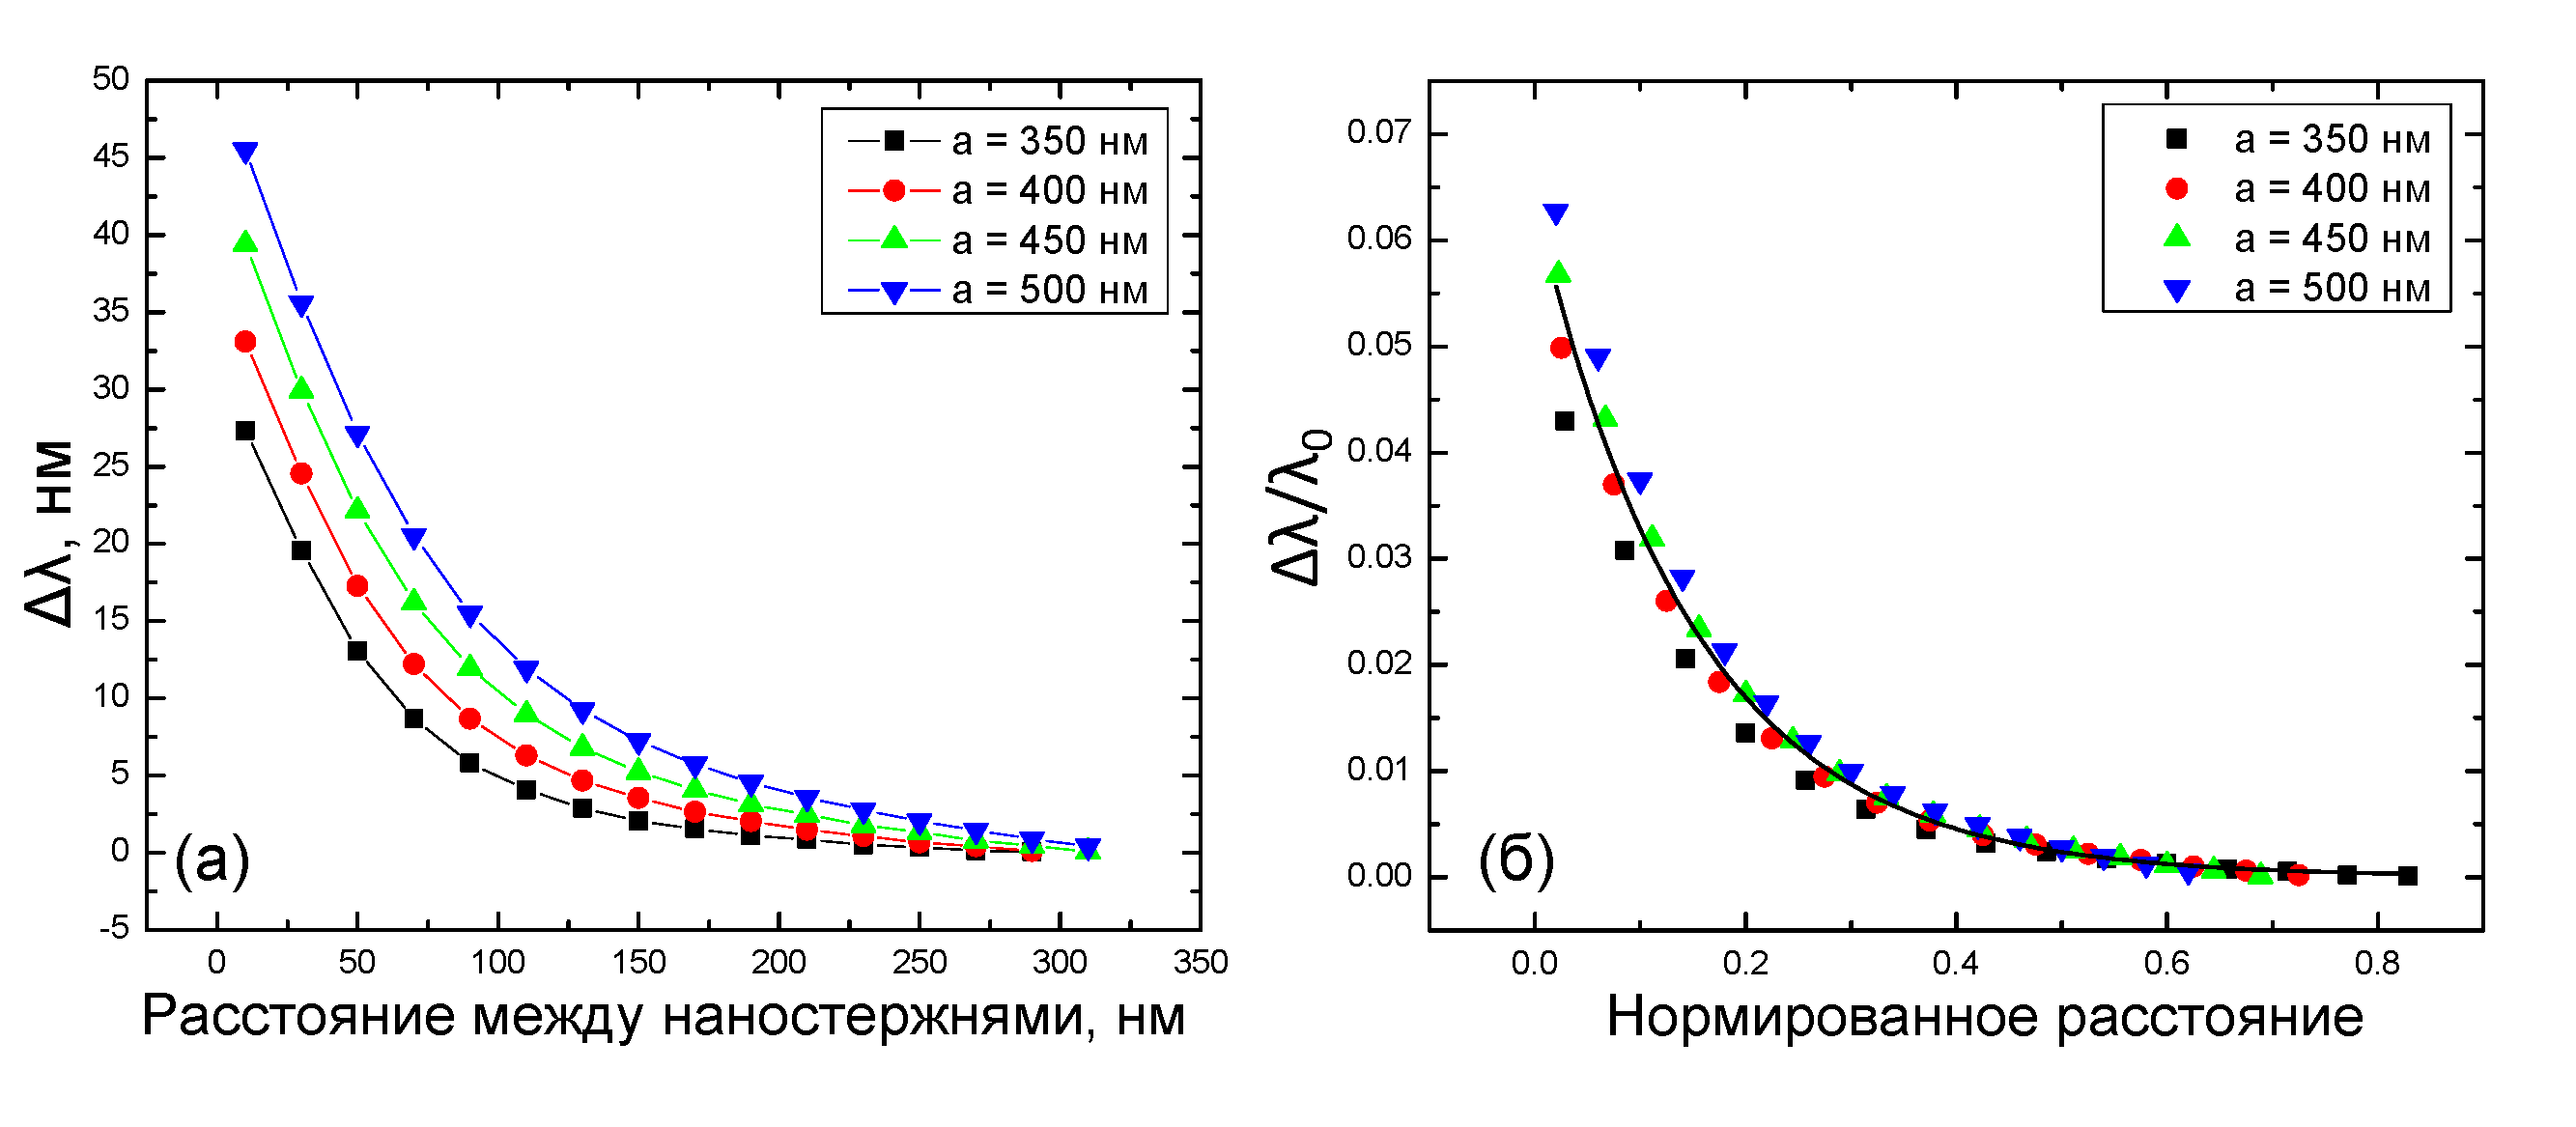
\includegraphics[width=16cm]{img/FDTD/ruler_res2.pdf}}
\caption{Графики зависимости сдвига резонанса второго порядка $ \Delta \lambda $ от расстояния между наностержнями (а) и зависимость относительного сдвига резонанса второго порядка от нормированного на длину  наностержня расстояния (б) при длине наностержней 350, 400, 450 и 500 нм }
\label{img:ruler2}
\end{figure}

Как правило, в экспериментальных исследованиях измеряется спектр не одиночной пары наночастиц, а ансамбля из пар наночастиц с фиксированным расстоянием между ними, как показано на рис.~\ref{img:PR_SEM}. Поэтому вместо граничных условий PML в плоскостях XZ и YZ были выбраны периодические граничные условия. Тогда размер интегрирования вдоль осей $ Ox $ и $ Oy $ можно интерпретировать как период между ансамблями спаренных наностержней. На рис.~\ref{img:BCperiod} показана зависимость коэффициента пропускания от длины волны и периода между ансамблями из спаренных наностержней. Видно, что положение резонанса также зависит и от периода между ансамблями из спаренных наностержней, что говорит о наличии дальнепольного дифракционного взаимодействия  вплоть до периода в 3 мкм. Для длины волны $ \lambda \approx 600$ нм наблюдается резонанс второго порядка, который менее чувствителен к периоду структуры.

\begin{figure}
\center{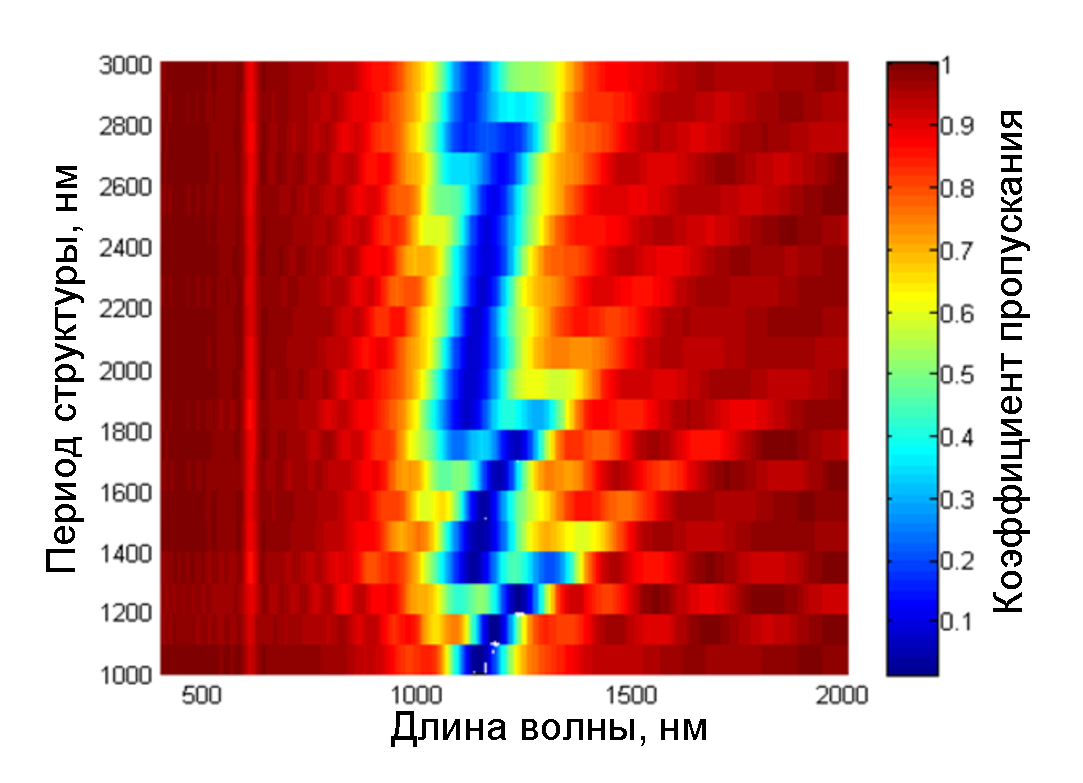
\includegraphics[width=10cm]{img/FDTD/BCperiod.pdf}}
\caption{График зависимости коэффициента пропускания от длины волны падающего электромагнитного излучения и периода между ансамблями из спаренных наностержней. Длина наностержней составляет 300 нм, а расстояние между ними -- 300 нм.}
\label{img:BCperiod}
\end{figure}

Таким образом, в результате численных расчетов  обнаружено наличие двух резонансов ЛПП  с различным локальным распределением плотности мощности для наностержней длиной до 500 нм, исследовано локальное распределение плотности мощности электромагнитного поля вблизи наностержней при резонансах различных порядков, а также на основе смещения положения резонансов первого и второго порядков были получены уравнения для <<плазмонных линеек>>.

